\documentclass{standalone}
\usepackage{tikz}
\usetikzlibrary{arrows.meta}
\begin{document}
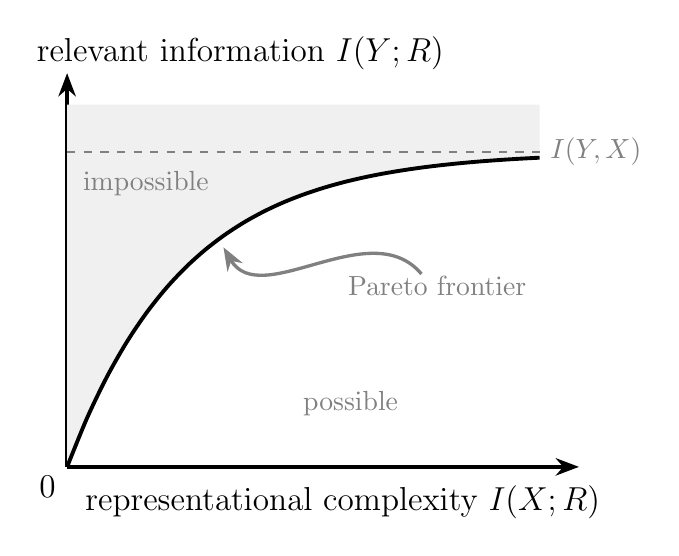
\begin{tikzpicture}[>=Stealth, line width=1.2pt, font=\large]
  % Axes
  \draw[->] (0,0) -- (6.5,0);
  \node at (3.5,-0.45) {representational complexity $I(X;R)$};
  % \node[text=gray] at (6.5,-0.6) {\footnotesize{more is better $\rightarrow$}};
  \draw[->] (0,0) -- (0,5);
  \node at (2.2,5.25) {relevant information $I(Y;R)$};
  % \node[text=gray] at (0,5.6) {\footnotesize{more is better $\uparrow$}};
  \node at (-0.25,-0.25) {$0$};
  % Impossible region (above the frontier)
  \fill[gray!12]
    (0,0)
    -- plot[domain=0:6, smooth, variable=\x] ({\x},{4*(1-exp(-\x/1.5))})
    -- (6,4.6) -- (0,4.6) -- cycle;
  % Pareto frontier
  \draw[line width=1.4pt]
    plot[domain=0:6, smooth, variable=\x] ({\x},{4*(1-exp(-\x/1.5))});
  % H(Y) asymptote
  \draw[gray, dashed, line width=1pt] (0,4) -- (6.05,4);
  \node[text=gray, anchor=west] at (6,4) {\normalsize{$I(Y,X)$}};
  % Region labels
  \node[text=gray] at (1.0,3.6) {\normalsize{impossible}};
  \node[text=gray] at (3.6,0.8) {\normalsize{possible}};
  % Pareto frontier label with leader
  \node[text=gray] at (4.7,2.3) {\normalsize{Pareto frontier}};
  \draw[gray, ->, shorten >=2pt] (4.5,2.45) to[out=130, in=300] (1.95,2.85);
\end{tikzpicture}
\end{document}
